\subsubsection{bringit::client::view::list::shareListWithGroup::ShareWithGroupView}

\label{bringit::client::view::list::shareListWithGroup::ShareWithGroupView}
\begin{figure}[H]
	\centering
	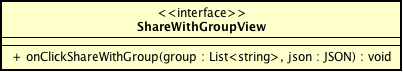
\includegraphics[scale=0.5]{Sezioni/SottosezioniST/img/app/ShareWithGroupView.png}
	\caption{bringit::client::view::list::shareListWithGroup::ShareWithGroupView}
\end{figure}

\begin{itemize}
\item \textbf{Descrizione}: La view relativa alla parte grafica di condivisione di una lista con un canale di ROcket.Chat.
\item \textbf{Utilizzo}: L'interfaccia viene utilizzata per disaccoppiare presenter e implementazione della classe e per visualizzare i dati che gli vengono passati dal presenter.
\item \textbf{Attributi}: 
\item \textbf{Metodi}:
	\begin{itemize}
	\item \textit{public onClickShareWithGroup():void}\\
	Questo metodo provvede alla condivisone di una lista con un canale di Rocket.Chat.
	\end{itemize}
\end{itemize} 

\subsubsection{bringit::client::view::list::shareListWithGroup::view::ShareWithGroupViewImpl}

\label{bringit::client::view::list::shareListWithGroup::view::ShareWithGroupViewImpl}
\begin{figure}[H]
	\centering
	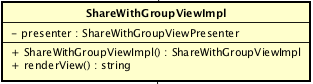
\includegraphics[scale=0.5]{Sezioni/SottosezioniST/img/app/ShareWithGroupViewImpl.png}
	\caption{bringit::client::view::list::shareListWithGroup::view::ShareWithGroupViewImpl}
\end{figure}

\begin{itemize}
\item \textbf{Descrizione}: Questa classe rappresenta la classe concreta di condivisione di una lista con un utente.
\item \textbf{Utilizzo}: Implementando i metodi di ShareWithGroupView questa classe viene utilizzata al momento della condivisone di una lista bringit con un canale di Rocket.Chat.
\item \textbf{Attributi}: 
\begin{itemize}
	\item \textit{private presenter:ShareWithGroupViewPresenter}\\
	Il presenter relativo alla condivisione di una lista con un canale di Rocket.Chat.
	\item \textit{private shareEmitter:ShareEventEmitter}\\
	Il riferimento all'oggetto responsabile dell'emissione degli eventi di condivisione di una lista.
\end{itemize}
\item \textbf{Metodi}:
	\begin{itemize}
	\item \textit{public ShareWithGroupViewImpl():ShareWithGroupViewImpl}\\
	Il costruttore di ShareWithGroupViewImpl.
	\item \textit{public onClickShareWithContact(group:string,json:JSONObject):void}\\
	Questo metodo provvede alla condivisone di una lista con uno specifico utente.
					\\ \textbf{Parametri}: \begin{itemize}
			\item \textit{group:string}\\
			Il nome del canale al quale si desidera condividere la lista.
			\item \textit{json:JSONObject}\\
			L'oggetto json contenente il messaggio che si desidera condividere.
					\end{itemize} 
	\end{itemize}
\end{itemize} 

\subsubsection{bringit::client::view::list::shareListWithGroup::presenter::ShareWithGroupViewPresenter}

\label{bringit::client::view::list::shareListWithGroup::presenter::ShareWithGroupViewPresenter}
\begin{figure}[H]
	\centering
	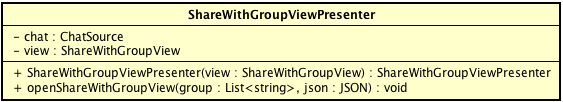
\includegraphics[scale=0.5]{Sezioni/SottosezioniST/img/app/ShareWithGroupViewPresenter.png}
	\caption{bringit::client::view::list::shareListWithGroup::presenter::ShareWithGroupViewPresenter}
\end{figure}

\begin{itemize}
\item \textbf{Descrizione}: Questa classe rappresenta il presenter per la classe di condivisione della lista bringit con un canale Rocket.Chat.
\item \textbf{Utilizzo}: Il presenter fa da tramite tra l'implementazione e la view, formattando i dati che verranno visualizzati nella view e manipolando gli input dell'utente per eseguire le operazioni logiche predisposte.
\item \textbf{Attributi}: 
	\begin{itemize}
	\item \textit{private chat:ChatSource}\\
	Il riferimento alla classe necessaria per interfacciarsi a Rocket.Chat.
	\item \textit{private view:ShareWithGroupView}\\
	La view necessaria al presenter.
	\item \textit{private popup:ShowPopupUseCase}\\
	Il riferimento all'oggetto necessario per il display di popup in Rocket.Chat.
	\end{itemize}
\item \textbf{Metodi}:
	\begin{itemize}
	\item \textit{public ShareWithGroupViewPresenter(view:ShareWithGroupView):ShareWithGroupViewPresenter}\\
	Il costruttore di ShareWithGroupViewPresenter.
					\\ \textbf{Parametri}: \begin{itemize}
			\item \textit{view:ShareWithGroupView}\\
			La view necessaria al presenter.
					\end{itemize} 
	\item \textit{public onClickShareWithContact(group:string,json:JSONObject):void}\\
	Questo metodo provvede alla condivisone di una lista con un canale Rocket.Chat.
					\\ \textbf{Parametri}: \begin{itemize}
			\item \textit{group:string}\\
			Il nome del canale al quale i desidera condividere la lista.
			\item \textit{json:JSONObject}\\
			L'oggetto json contenente il messaggio che si desidera condividere.
					\end{itemize} 
	\end{itemize}
\end{itemize} 
 
 
